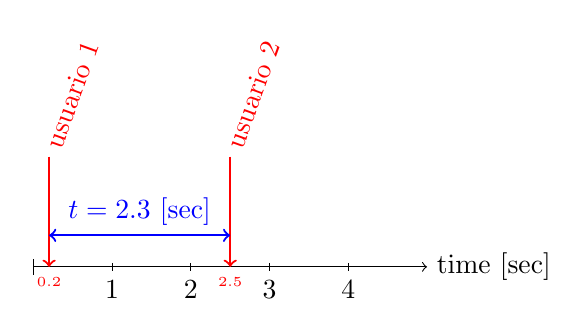
\begin{tikzpicture}
    % Time axis
    \draw[|->] (0,0) -- (5,0) node[anchor=west] {time [sec]};

    % ticks
    \draw (1,.05) -- (1,-.05) node[below] {1};
    \draw (2,.05) -- (2,-.05) node[below] {2};
    \draw (3,.05) -- (3,-.05) node[below] {3};
    \draw (4,.05) -- (4,-.05) node[below] {4};

    
    % arrivals
    \draw[->,color=red,thick] (0.2,1.4) node[anchor=west,rotate=70] {usuario 1} --(0.2,0) node[below,anchor=north] {\tiny 0.2};
    \draw[->,color=red,thick] (2.5,1.4)node[anchor=west,rotate=70] {usuario 2} --(2.5,0) node[below,anchor=north] {\tiny 2.5};

    \draw[<->,color=blue,thick] (0.2,.4) -- node[above,pos=0.5]{$t=2.3$ [sec]} (2.5,.4);
\end{tikzpicture}
